%%%%%%%%%%%%%%%%%%%%%%%%%%%%%%%%%%%%%%%%%%%%%

\section{Previous Work}
\label{sec:PreviousWork}
Previous work on the energy deposition of thin focused on spectra measurements from fabricated films as wells as single collision energy loss spectra.
A sequence of 10\% \iso{Li}{6}F, 5\% PPOPOPOP films in a PS matrix cast to thickness between 15 and 600 $\mu$m where fabricated and the response was measured from a gamma source as well as a neutron source.
These experiment results are shown in \ref{sec:SpectraMeasurements}.


\subsection{Spectra Measurements}
\label{sec:SpectraMeasurements}
Evidence that the secondary electrons contribute to energy loss can be seen in Figure \ref{fig:SpectraFeatures} where there is an increase in the endpoint of the spectra as films become thicker.
This increase in the spectra endpoint is indictive of the film producing more light, and as the light collection geometry remained constant the increase in the endpoint is attributed to a larger energy deposition in the 50 $\mu$m film compared to the 15 $\mu$m or 25 $\mu$m film.
%%%%%%%%%%%%%%%%%%%% Figures %%%%%%%%%%%%%%%%%%%%%%%%
\begin{figure}
    \centering
    \caption{Spectra properties as a function of film thickness}
    \begin{subfigure}[b]{0.45\figurewidth}
        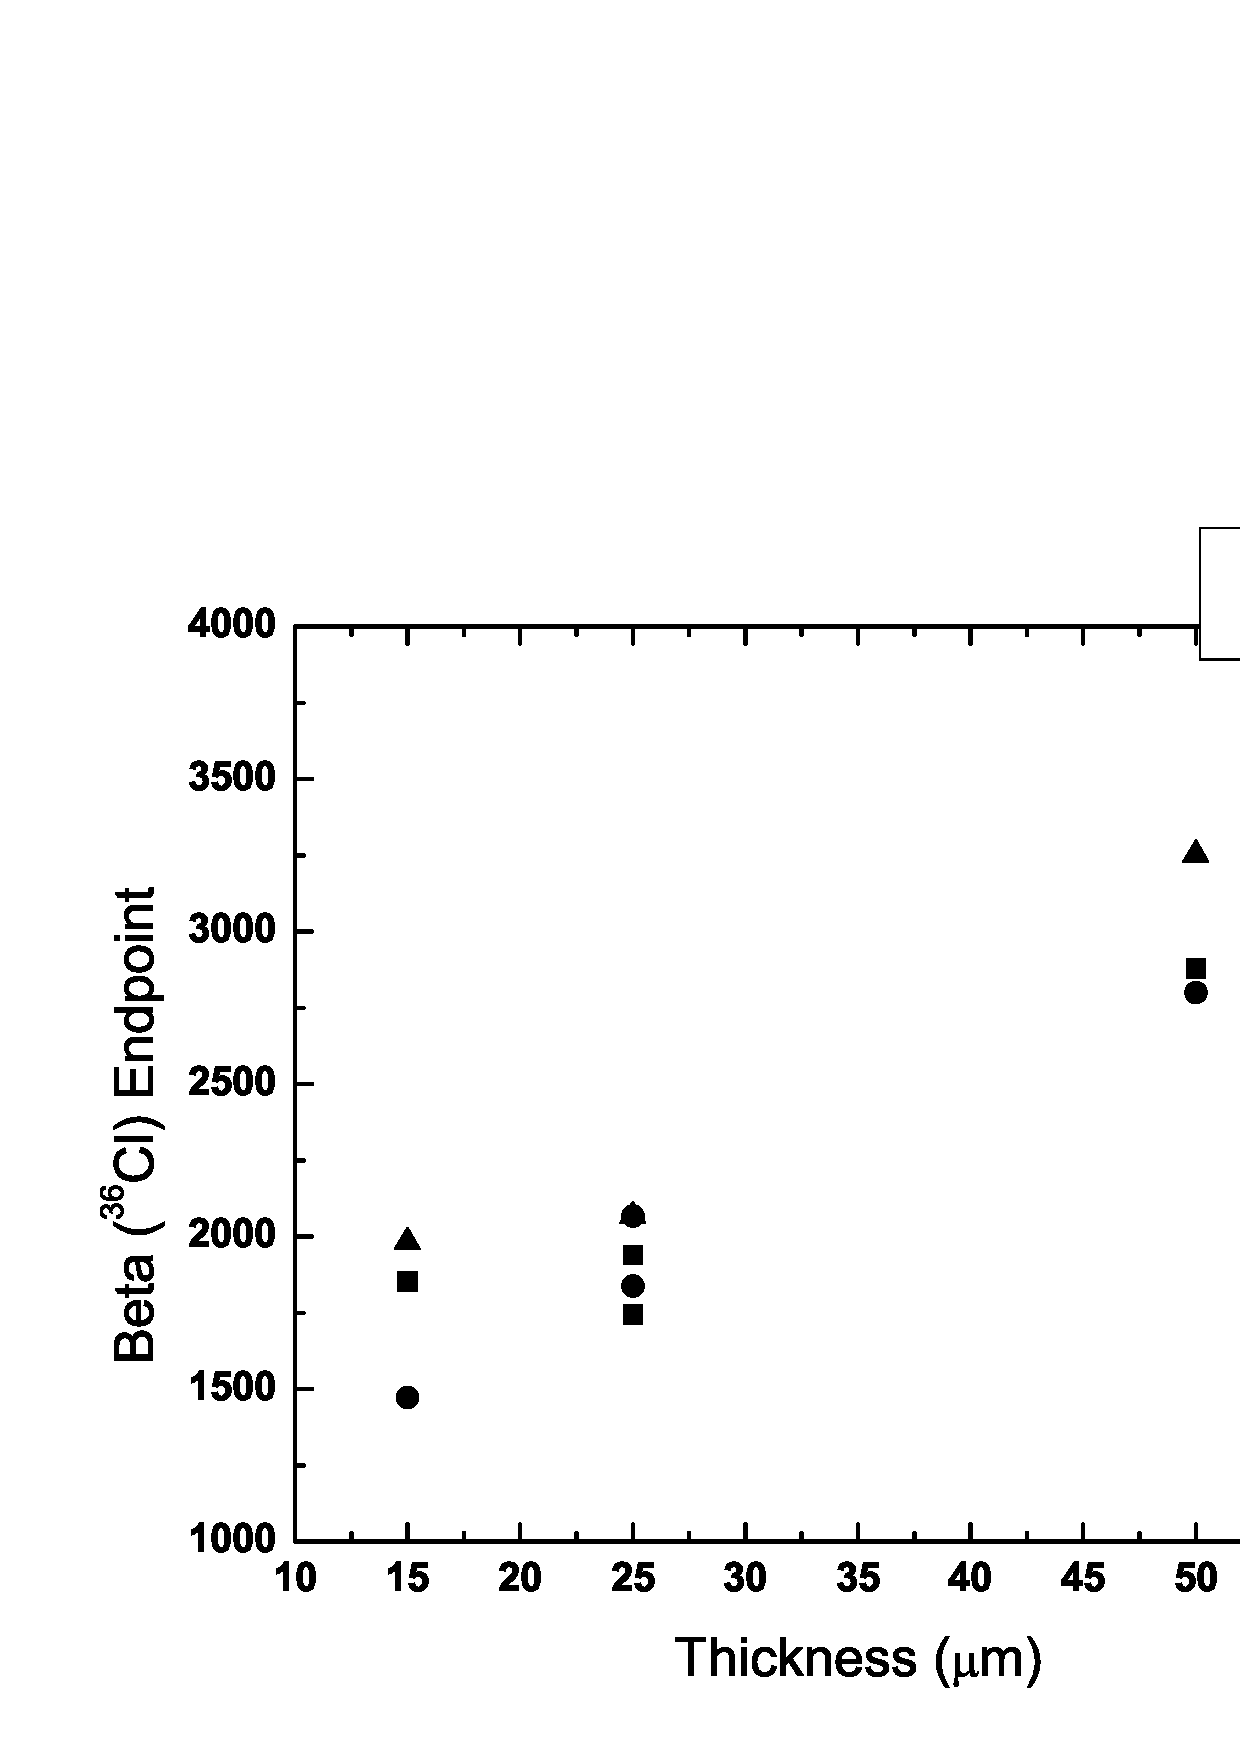
\includegraphics[width=\textwidth]{Beta}
        \caption{Beta Spectra Endpoints for a 5\% PS film}
    \end{subfigure}
    \begin{subfigure}[b]{0.45\figurewidth}
        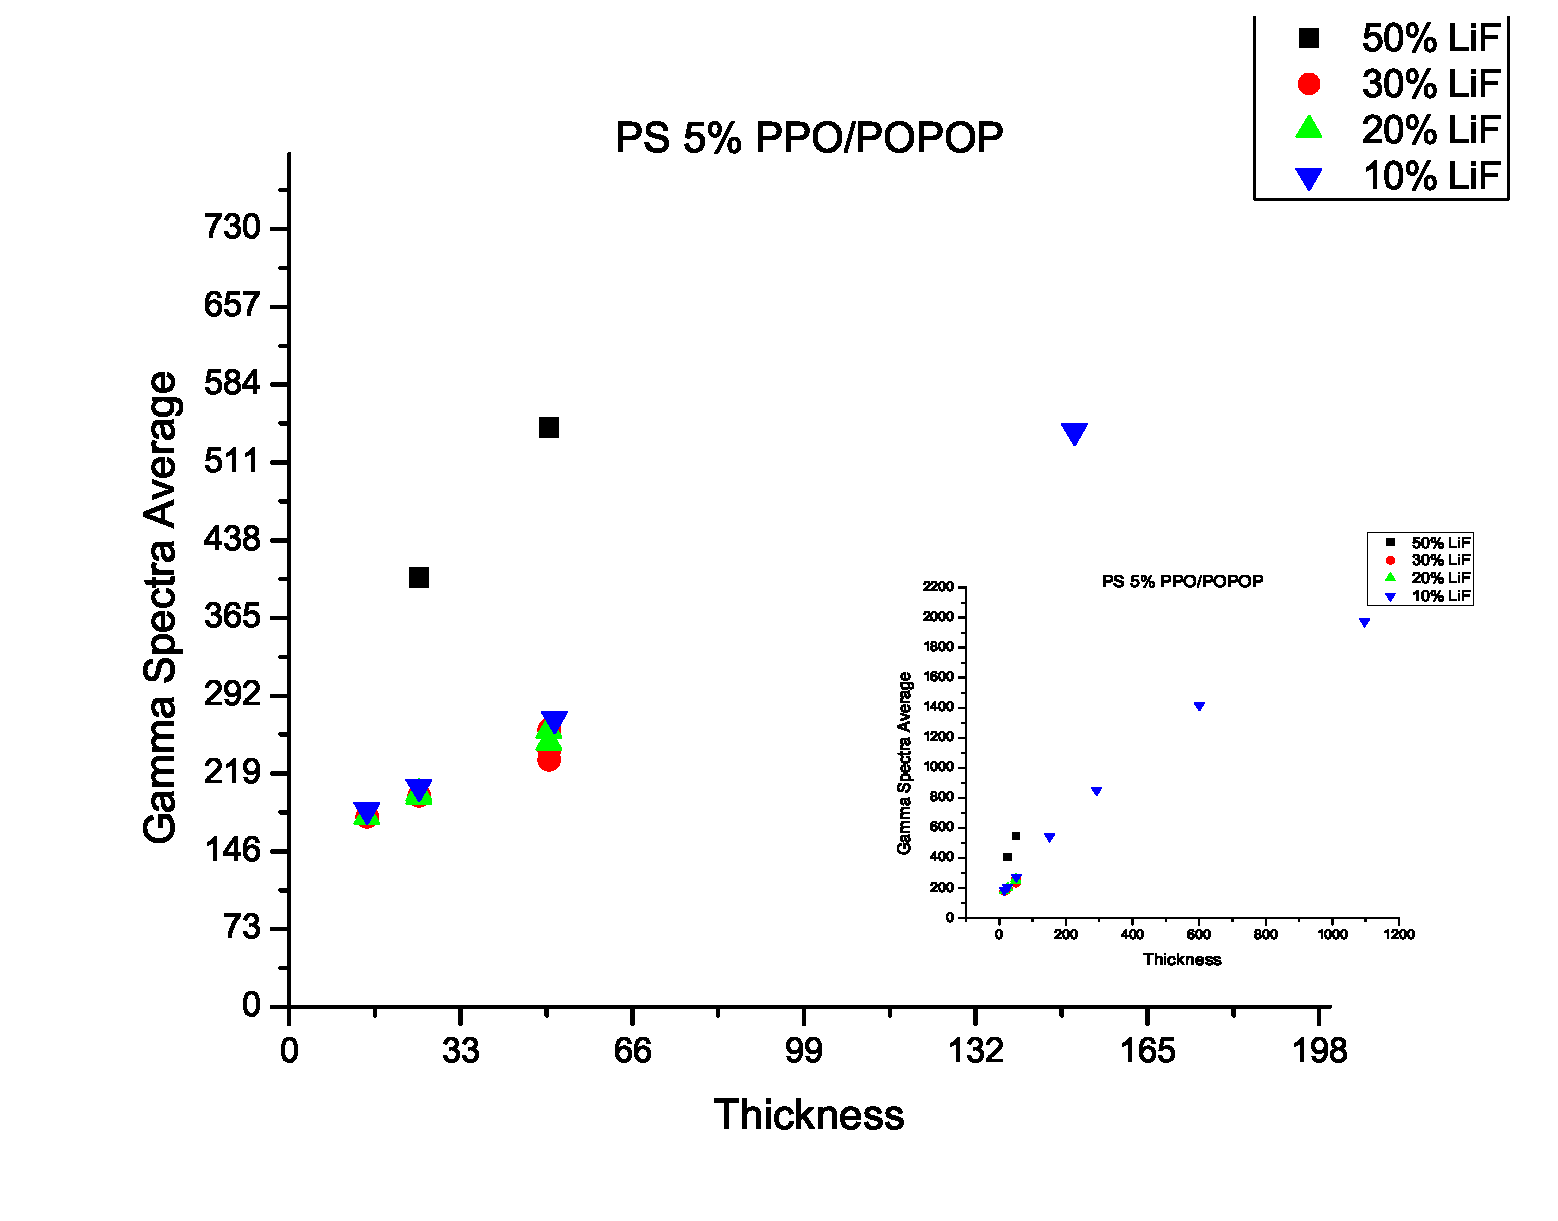
\includegraphics[width=\textwidth]{PS-5PPOPOPOP_GammaAvg}
        \caption{Gamma Spectra Averages for PS films}
    \end{subfigure}
    \label{fig:SpectraFeatures}
\end{figure}
Figure \ref{fig:GammaIntrNeutronCounts} shows the intrisinic efficiency of these film (from spectra obtained from a \iso{Co}{60} source).
As the film thickness increases the pulse height discriminator at which an intrisinic efficiency of one in a million ($\epsilon_{int,\gamma} \le 10^{-6}$) is reached also increase.
The neutron spectra (shown in the solid lines) does not increase in light yield with increasing thickness, further providing an indication that the thickness of the films can be optimized to maximize the neutron count rates\footnote{The neutron count rate is increased with thickness by the increased mass of the detector} while minimizing the response of the detector to photons.
%%%%%%%%%%%%%%%%%%%% Figures %%%%%%%%%%%%%%%%%%%%%%%%
\begin{figure}
    \centering
    \caption{Gamma intrinsic efficiency (dashed lines) plotted against neutron counts (solid)}
    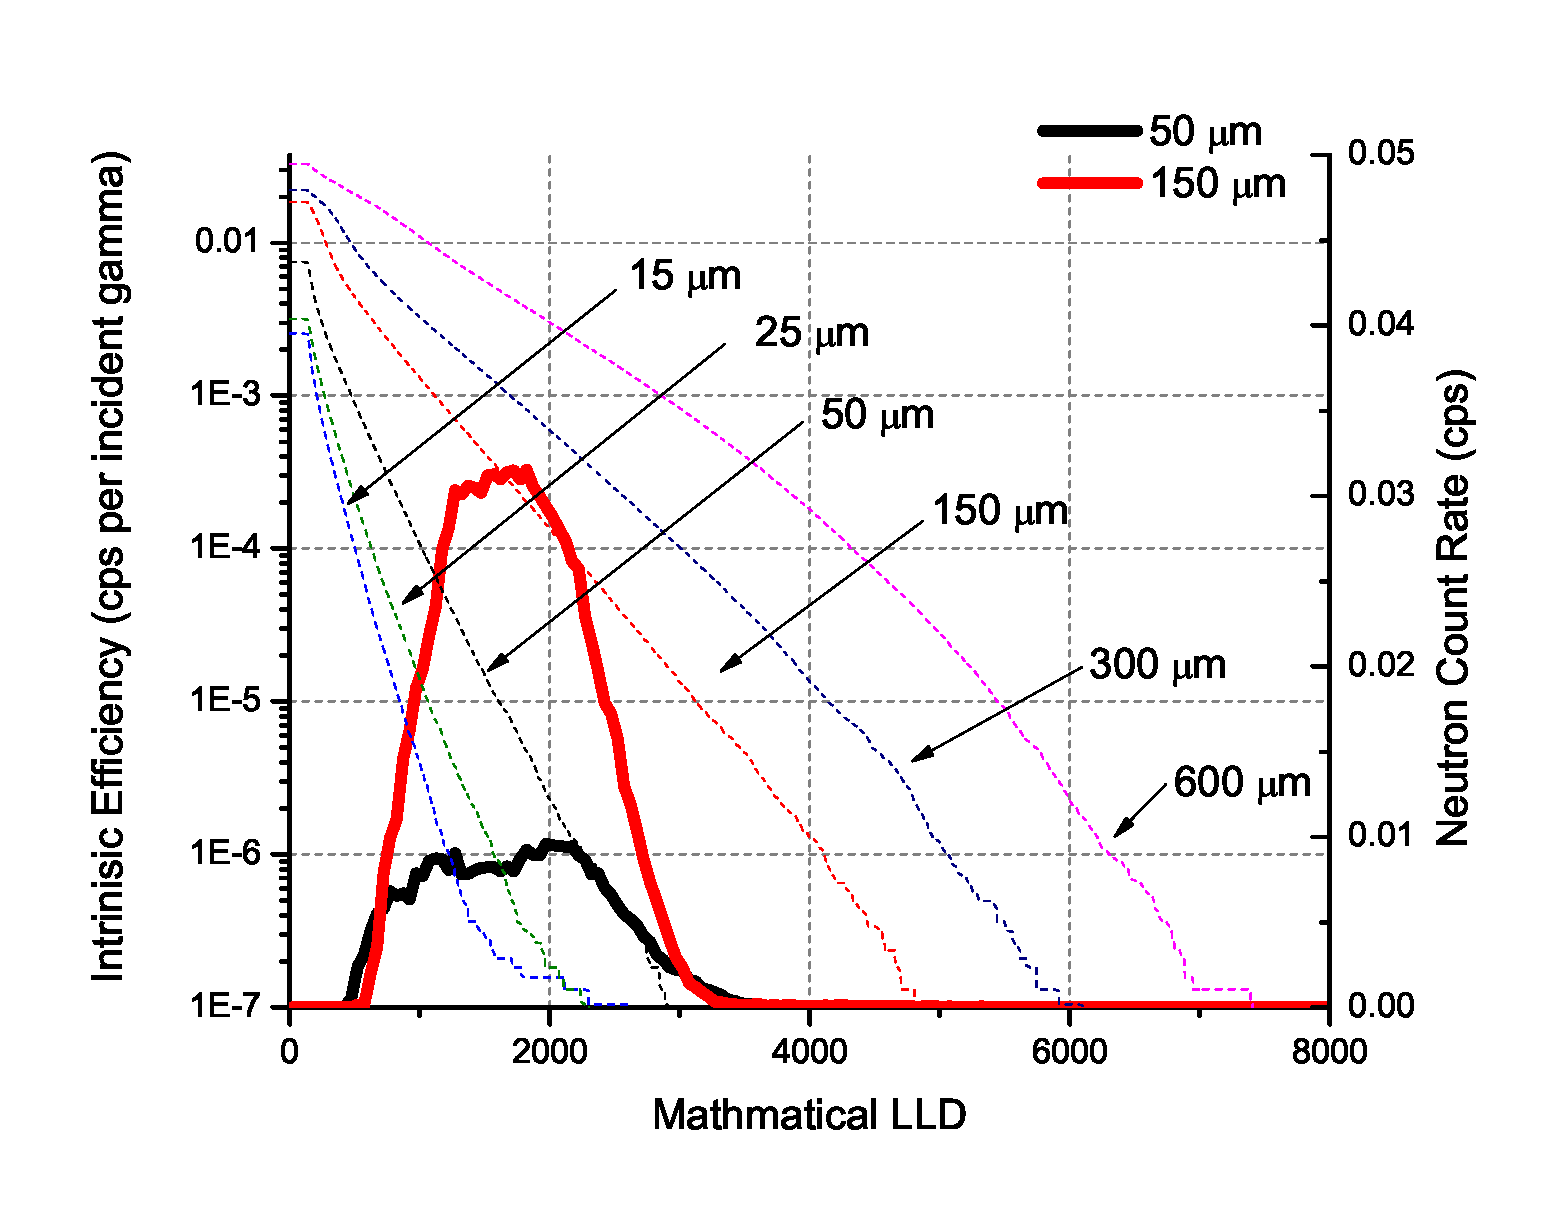
\includegraphics[width=\textwidth]{PS_IntEff_LiF20_PPO5}
    \label{fig:GammaIntrNeutronCounts}
\end{figure}

